\documentclass[10pt]{article}
\usepackage[utf8]{inputenc}
\usepackage{geometry} % to change the page dimensions
\geometry{a4paper}
\usepackage{authblk}

%% Packages
\usepackage{graphicx, subcaption}
\usepackage{amsmath,amssymb,amsthm,amsfonts}
\usepackage{bm}
\usepackage{algorithm, algorithmic}
\usepackage{multirow}
\usepackage{bbm}
\usepackage{hyperref}
\usepackage{kotex}
\usepackage[labelformat=simple]{subcaption}

\usepackage{tikz}
\usetikzlibrary{shapes.geometric, arrows, positioning, calc}
\usetikzlibrary{backgrounds}

\tikzstyle{title} = [rectangle, minimum width=3cm, minimum height=1cm, text centered, draw=black, text width=3cm, fill=white!100]
\tikzstyle{startstop} = [rectangle, rounded corners, minimum width=3cm, minimum height=1cm,text centered, draw=black, fill=red!30]
\tikzstyle{io} = [trapezium, trapezium left angle=70, trapezium right angle=110, minimum width=3cm, minimum height=1cm, text width=1.3cm, text centered, draw=black, fill=blue!30]
\tikzstyle{process} = [rectangle, minimum width=3cm, text width=3cm, minimum height=1cm, text centered, draw=black, fill=orange!30]
\tikzstyle{decision} = [diamond, minimum width=3cm, minimum height=1cm, text centered, draw=black, fill=green!30]
\tikzstyle{arrow} = [thick,->,>=stealth]

\captionsetup[figure]{labelsep=period}
\renewcommand{\thefigure}{\Roman{figure}}
% \captionsetup[subfigure]{labelformat=parens} % default is 'parens'
% \renewcommand{\thesubfigure}{\thefigure.\alph{subfigure}.}
\renewcommand\thesubfigure{(\alph{subfigure})}

%% Theorems
\theoremstyle{plain}
\newtheorem{theorem}{Theorem}[section]
\newtheorem{proposition}[theorem]{Proposition}
\newtheorem{lemma}[theorem]{Lemma}

\theoremstyle{remark}
\newtheorem{remark}[theorem]{Remark}
\newtheorem{example}[theorem]{Example}

\theoremstyle{definition}
\newtheorem{definition}[theorem]{Definition}

%% Equations
\numberwithin{equation}{section}

%% Algorithms
\renewcommand\algorithmicdo{}
\renewcommand\algorithmicthen{}
\renewcommand\algorithmicendfor{\textbf{end}}

%% Macros
\def\chfun{\mathbbm{1}}
\def\skel{\mathcal{S}}
\def\calc{\mathcal{C}}
\def\sko{\hat{\mathcal{S}}}
\def\ske{\mathcal{S}^8}
\def\endske{E\left(\mathcal{S}^8\right)}
\def\endomc{E\left(\Omega_c\right)}


\def\gphi{\nabla\phi}
\def\ngphi{\left|\nabla\phi\right|}
\def\ngphii{\left|\nabla\phi_i\right|}
\def\fci{F_{c,\,i}}
\def\fcj{F_{c,\,j}}
\def\cm{\, ,}
\def\pd{\, .}

\def\omi{\Omega_i}
\def\oma{\Omega_a}
\def\ome{\Omega_E}
\def\omc{\Omega_c}
\def\omcc{\hat{\Omega}_c}

\def\sdf{\mbox{SDF}}

\DeclareMathOperator*{\argmax}{arg\,max}
\DeclareMathOperator*{\argmin}{arg\,min}
% \def\tOmega{\tilde{\Omega}}
% \def\tGamma{\tilde{\Gamma}}
% \def\tV{\tilde{V}}
% \def\W{\mathbb{W}}
% \def\tu{\tilde{u}}
% \def\bu{\bar{u}}
% \def\hu{\hat{u}}
% \def\bl{\bar{\lambda}}
% \def\p{\mathbf{p}}
% \def\P{\mathbf{P}}
% \def\intO{\int_{\Omega}}
% \def\intOs{\int_{\Omega_s}}
% \def\m{\mathbf{m}}
% \def\n{\mathbf{n}}
% \def\blambda{\bm{\lambda}}

% \def\tE{\tilde{E}}
% \def\N{\mathcal{N}}

% \def\div{\mathrm{div}}
% \def\proj{\mathrm{proj}}
% \def\prox{\mathrm{prox}}
% \def\ran{\mathrm{ran}\,}
% \def\ed{\mathrm{ed}}
% \def\supp{\mathrm{supp}\,}
% \def\TOL{\mathrm{TOL}}
% \DeclareMathOperator*{\argmin}{\arg\min}

% Text Color and Strike
\usepackage[normalem]{ulem}
\usepackage{color}
\newcommand{\red}[1]{{\color{red}{#1}}}
\newcommand{\blue}[1]{{\color{blue}{#1}}}

\title{Individual Tooth Segmentation in 2D Human Teeth Image}
\author{Seongeun Kim and Chang-Ock Lee}
\affil{Department of Mathematical Sciences, KAIST, Daejeon 34141, Korea}
\date{2022-01-01}

\begin{document}
\maketitle

\begin{abstract}
Reconstruction of 3D teeth from a 2D human teeth image is considered a difficult problem and required in many fields such as computer graphics and personal health cares. In a recent study \cite{WU:2016}, a method for reconstructing 3D teeth from individual tooth regions of a 2D human teeth image was proposed. 
However, obtaining individual tooth regions from a 2D human teeth image is very difficult due to common obstacles: weak edges, intensity inhomogeneities and strong light reflections. In this study, we present a method of segmenting individual tooth regions from a 2D human teeth image under the active contour framework, by acquiring candidates for edge regions despite such obstacles using a deep neural network (DNN). We also present a strategy for using classical image processing methods to streamline the data labeling process and training deep neural networks.
\end{abstract}

{\small \textbf{Key words}
Image Processing, Neural Networks, Data Processing}

{\small \textbf{AMS subject classifications}
94A08, 68T07}

%% Main text starts ---------------------------------------------------------------------------------------------------
% Section: Introduction
\section{Introduction}
\label{Sec:Introduction}

Extracting 3D teeth model is very important technique required in various fields. In the medical fields, plaster model or an intra oral scanner is mainly used for obtaining a precise 3D teeth model. These methods not only require the help of a professional, but are also time consuming and costly. In the computer graphics, although it is not completely identical to the real teeth, methods that can obtain 3D teeth model more easily and in various ways are also required. The most common examples are reconstruction of 3D teeth from 2D CT images of teeth \cite{Naumovich:2015,Yuan:2020}. In \cite{WU:2016}, a 3D teeth model reconstruction using a single 2D teeth image was proposed. The segmentation is done by extracting tooth boundaries in the 2D image: after setting a parametric model of the 3D teeth rows, and then find optimal parameters fit to the extracted tooth boundaries. Considering these results, we can know that if the individual tooth regions of the 2D teeth image are well segmented, then a 3D teeth model can be reconstructed as well as the 2D teeth image not only contains some information about the entire 3D teeth rows. In \cite{WU:2016}, a supervised learning method BEL \cite{Dollr:2006} was used to obtain the individual tooth boundaries, and manually labeled $40$ teeth studio-taken images are used as the training data. In the supervised learning method, it is a well-known fact that in order for a model to perform stably, a sufficient amount of training data with diversity is required. However, if labeling process takes a lot of time and cost, it becomes difficult to produce such dataset and this inevitably limits the performance and range of the model. With this in mind, we propose a method for individual tooth segmentation from a mobile phone-level 2D tooth image, and we approached it in the context of minimizing human touch by using model-based image processing methods. Some attempts have been made to segment individual tooth from a 2D teeth image. In \cite{LeeColor:2009,LeeWater:2010} it was tried by using the color information and the watershed algorithm. In \cite{LeeRemoval:2010,LeeSegRemoval:2010}, an additional light reflections removing process was applied before segmentation. In very recent studies \cite{Pham:2020,Kim:2020,Zhu:2020}, direct segmentations using deep learning methods have been proposed, and all of these studies were done through learning of Mask R-CNN \cite{He:2018}.

Putting these aside for a moment, let us make a brief mention about image segmentation. The image segmentation is one of the large and major topic in the field of computer visions. The main goal of image segmentation is to precisely capture objects in an image according to a specific purpose, and many outstanding methodologies have been developed. The active contours model is one of the popular method for the image segmentation, which makes contour moving forward to the boundary of objects. To this end, early active contour models worked hard to design forces that moves the contour to the desired edge. A model that is a pioneer in active contours is \cite{Kass:1988} and from this, a lot of brilliant progresses have occurred. The gradient vector flows \cite{Xu:1997}, geodesic active contours \cite{Caselles:1997} and balloon forces \cite{COHEN:1991} are generally well-known models. In \cite{Chan:2001}, a novel and remarkable method was proposed which does not extract edge during the segmentation. There are also statistical models that forces contour to region which has more similar intensities \cite{Zhu:1996,Park:2014}. In the \cite{Park:2014} a statistically reinstating method (SRM) was proposed, and the force $F_s$ is defined for the method. Since the force $F_s$ moves the contour using three distinct regions of difference scales, it can approach to fit clear edge even for a variety of resolutions. 

Returning to the main topic, in this paper, we try to segment individual tooth regions through active contours. In order for the contours to form each tooth boundary well, first, it must be possible to detect the precise edge when the contour approaches the boundary and secondly, there should be no factors interfering the contour. Furthermore in natural images, there are boundaries that cannot be detected by intensity alone,even for there tooth boundaries should be decided to form closed tooth regions. With these considerations in mind, we propose the edge region candidate $\omc$ and competing balloon force $F_{c,\,i}$ with a contour evolution in a level set formulation:
\begin{align}
    \frac{\partial}{\partial{t}}\phi_i(x,\,t) &= \mu\kappa(\phi_i)\ngphii + \chi_{\Omega\setminus\ome}\fci\ngphii+\chi_{\omc\setminus\ome}F_s\ngphii-\chi_{\omc\cap\ome}F_a\cdot \gphi \cm \label{Eq:proposed}\\
    \phi_i(x,\,0) &= \phi_{i,\,0}\cm \nonumber
\end{align}
where $\mu$ is a constant, $\Omega$ is the given image domain, $\chi_A$ is the characteristic function of the subscribed set $A$ and $\kappa(\phi_i)$ is curvature of a signed distance function (SDF) $\phi_i$. The unexplained two sets $\omc$, $\ome$ and one force $F_a$ will be elaborated in the Section~\ref{Subsec:GADF}. Here, the force $F_s$ of SRM is used with slight modifications from the original text \cite{Park:2014}. Originally, it makes a balloon force on where the distributions of image intensities of both sides of the contour are relatively similar, but we have repeated balloon force in $F_{c,\,i}$ and thus we omitted the balloon force from $F_s$.

For the remainder of this paper, we denote $\sdf(X)$ or $\sdf$ of a set $X$ as a signed distance function which is negative on the set $X$ and constantly zero on $\partial X$. Further, $S_\omega(x)$ means a $\omega\times\omega$ window centered at $x$.

% Sec:Background
\section{Background}
\label{Sec:BG}
In this section, we briefly review geometric attraction-driven flow (GADF) \cite{Hahn:2006, Hahn:2010} and edge region, which plays important role for segmenting individual tooth. We will derive how to obtain edge regions by concerning the problematic features of teeth image.

% Subsec:GADF
\subsection{Geometric Attraction-Driven Flow}
\label{Subsec:GADF}
Assume there is a smooth gray image $I:\Omega\subset\mathbf{R}^2\rightarrow[0,\,1]$. The image intensity changes rapidly on the boundary of two objects in the image. Thus, we define a point $x\in\Omega$ as an edge of the image if
\begin{align}
    % \left.u_x''(s)\right|_{s=0}=0\cm \label{Def:edge}
    u_x''(0)=0\cm \label{Def:edge}
\end{align}
where
\begin{align*}
    u_x(s) = I\left( x + s\frac{\nabla{I(x)}}{|\nabla{I(x)}|} \right)\pd
\end{align*}
The GADF is defined as
\begin{align}
    F_a(x) = \mbox{sgn}(\ell(x))\frac{\nabla I(x)}{\left|\nabla{I(x)}\right|},\quad \forall{x}\in\Omega\cm  \label{Def:gadf}
\end{align}
where the $\mbox{sgn}$ is the sign function and 
\begin{align*}
    \ell(x) &= \int^{\epsilon}_{0} {u'_x(s)}\,ds - \int^{0}_{-\epsilon} {u'_x(s)}\,ds\quad\mbox{for a small}~\epsilon > 0\cm
\end{align*}
By the definition, $F_a(x)$ directs the edges on the line $x + s\frac{\nabla{I(x)}}{|\nabla{I(x)}|}$ that is the points on which $u_x''(s)=0$. 

An edge region means a region where an edge is thought to exist. In \cite{Hahn:2010}, edge region is defined by using regions where $F_a$ are facing each other, i.e.
\begin{align}
    \Omega_a = \delta_{S_3}\left( \Omega_E \right)\cm \label{Def:edge_region}
\end{align}
where $\delta_{S_3}$ is a dilation function using $S_3$ and 
\begin{align}
    \Omega_E = \left\{ x\in\Omega \mid F_a(x^*) \cdot F_a(x) < 0 ~\mbox{and}~ x^*=x+F_a(x) \right\}\pd \label{Def:pre_er}
\end{align}
Under this setting, contour evolution using a level set formulation is proposed:
\begin{align}
    \frac{\partial}{\partial{t}}\phi(x,\,t) &= \mu\kappa(\phi)\left|\nabla\phi\right| - \chi_{\oma}F_a\cdot\nabla\phi + \chi_{\Omega_b}F_b|\nabla\phi|\cm \label{Eq:gadf}\\
    \phi(x,\,0) &= \phi_0(x)\cm \nonumber
\end{align}
where $\alpha$ is a constant, $\phi$ is initial $\sdf$. Observe that initial contour approaches the edge in $\Omega_a$ by $F_a$ and goes outward in $\Omega_b = \Omega\setminus\Omega_a$ by a balloon force $F_b$.

The GADF is naturally expandable with color images. For a color image $I:\Omega\subset\mathbf{R}^2\rightarrow[0,\,1]^3$, we can consider a nonlinear structure tensor $\mathbf{M}$ from a nonlinear diffusion
\begin{align*}
    \frac{\partial \mathbf{M}(x,\,t)}{\partial t}&=\nabla\cdot\left( h\left( \sum_{i,\,j=1}^2 \left|\nabla M_{ij}(x,\,t)\right|^2  \right) \nabla\mathbf{M}(x,\,t) \right)\cm\\
    \mathbf{M}(x,\,0) &= \sum_{k=1}^3 {\nabla I_k(x)I_k(x)^T}\cm
\end{align*}
and the diffused tensor $\mathbf{M}$ preserves local features of the image $I$ \cite{Rousson:2003, Weickert:2004, Brox:2006, Hahn:2009}. We can count the eigenvector with respect to the maximum eigenvalue of $\mathbf{M}$ as a gradient of the color image $I$ and then the defining GADF is tractable.

% Subsection: Weak edge detection
\subsection{Weak edge detection}
\label{Subsec:weakedge}
When the change of intensity at the edge of an image is smaller than the neighborhood, we call it a weak edge. For a gray image $I$,
\begin{align*}
    \nabla{|\nabla{I(x)}|} \parallel \mathcal{H}_x(I)\nabla{I}(x)  
\end{align*}
is easily obtained from calculations, and it show that the direction of $\nabla|\nabla{I}|$ is getting differ to the $\nabla{I}$ whenever change of intensities is smaller than neighborhood, because of the affection of the hessian matrix $\mathcal{H}_x(I)$ ax $x$. In other words, around weak edges, it is difficult to determine the edge or edge region by simply using intensities. However, as can be seen in \eqref{Def:gadf}, GADF is defined to have one of the directions of $\nabla{I}$ and $-\nabla{I}$, and thus it is possible to find an edge region that includes all weak edges regardless of the amount of intensity change. Weak edges are common in human teeth images. In particular, it appears at the boundary between the teeth and the gums, boundary between two teeth with similar color and brightness or the joints of boundaries. Figure~\ref{Fig:weak_edges} shows the weak edges seen in the tooth image and the edges or edge regions detected by different methods.

% Figure: Weak edges in teeth image
\begin{figure}
    \centering
    \begin{subfigure}{1\textwidth}
        \centering
        \includegraphics[width=10cm]{./Figures/Fig1_img.png}
        \caption{A whole teeth image}
        \label{fig:1a}
    \end{subfigure} 
    \newline 
    
    \vspace{1mm}
    
    \begin{subfigure}{.18\textwidth}
        \centering
        \includegraphics[width=2.6cm]{./Figures/Fig1_img1.png}
        \includegraphics[width=2.6cm]{./Figures/Fig1_img2.png}
        \includegraphics[width=2.6cm]{./Figures/Fig1_img3.png}
        \caption{}
    \end{subfigure}
    \begin{subfigure}{.18\textwidth}
        \centering
        \includegraphics[width=2.6cm]{./Figures/Fig1_sbl1.png}
        \includegraphics[width=2.6cm]{./Figures/Fig1_sbl2.png}
        \includegraphics[width=2.6cm]{./Figures/Fig1_sbl3.png}
        \caption{Sobel}
    \end{subfigure}
    \begin{subfigure}{.18\textwidth}
        \centering
        \includegraphics[width=2.6cm]{./Figures/Fig1_cny1.png}
        \includegraphics[width=2.6cm]{./Figures/Fig1_cny2.png}
        \includegraphics[width=2.6cm]{./Figures/Fig1_cny3.png}
        \caption{Canny}
    \end{subfigure}
    \begin{subfigure}{.18\textwidth}
        \centering
        \includegraphics[width=2.6cm]{./Figures/Fig1_er1.png}
        \includegraphics[width=2.6cm]{./Figures/Fig1_er2.png}
        \includegraphics[width=2.6cm]{./Figures/Fig1_er3.png}
        \caption{$\ome$}
        \label{Fig:1d}
    \end{subfigure}
    \caption{(a) A whole teeth image and (b) sub-images in the red boxes. The results of various methods are shown. (c - d) Sobel and Canny edge detector with automatically chosen thresholds by MATLAB \cite{MATLAB:R2021a_u1}. (e) $\Omega_E$ from the GADF. }
    \label{Fig:weak_edges}
\end{figure}
    
% Subsection: Edge regions outside the tooth boundaries
\subsection{Edge regions outside the tooth boundaries}
\label{Subsec:eroutside}

In reality, teeth image contains various edges appeared outside of the tooth boundary due to inhomogeneities of the object surface or noise present in the image. Because of these edges, $\oma$ from GADF includes many connected regions outside the tooth boundary, as shown in Figure~\ref{Fig:1d}. These outside regions prevent the contours from getting closed to the tooth boundaries, so we have to handle them. They can be roughly divided into three categories according to the causes:
\begin{itemize}
    \item [(1)] Noise or small stains,
    \item [(2)] Large and faded stains having some clear parts,
    \item [(3)] Strong specular reflections.
\end{itemize} 
The regions caused by the tooth boundary are supposed to very large and colors of the image are changed rapidly around them. On the other hand, the edge regions caused by (1) are small and the colors are relatively flat, thus they can be removed by priority \cite{Hahn:2006}. (2) Some stains on the image makes a relatively large edge region. It is not easy to distinguish these regions from edge regions on the tooth boundary only by size and color information. However, if not all of the stains is clear and there is some faded parts, then the end of the edge region in that part is exposed. As the initial contour evolves by \eqref{Eq:gadf}, if it meets the ends, then it shrinks along the GADF and because of the curvature term, and so the edge regions arising from (2) can be canceled out. On the other side, edge regions arises from (3) are in large and closed shape. Because of the shape in which the ends are not exposed, it cannot be handled like (2). These edge regions block the move of the contour like a barrier and makes it difficult to find the correct tooth boundary. As a result, they are being main obstacles of the individual tooth segmentation. Contour evolution around the various shaped regions are appeared in Figure~\ref{Fig:er_outside}.

% Figure: Edge regions outside the tooth boundaries
\begin{figure}
    \centering
    % First row
    \begin{subfigure}{.24\textwidth}
        \centering
        \includegraphics[height=2.8cm]{./Figures/Fig2_img.png}
        \caption{}
        \label{Fig:2a}
    \end{subfigure}
    \begin{subfigure}{.24\textwidth}
        \centering
        \includegraphics[height=2.8cm]{./Figures/Fig2_er.png}
        \caption{}
        \label{Fig:2b}
    \end{subfigure}
    \begin{subfigure}{.24\textwidth}
        \centering
        \includegraphics[height=2.8cm]{./Figures/Fig2_reser.png}
        \caption{}
        \label{Fig:2c}
    \end{subfigure}\\
    \vspace{1mm}
    % First row
    \begin{subfigure}{.025\textwidth}
        \centering
        \caption*{\rotatebox[origin=c]{90}{\hspace{-4mm} (d) Left tooth}}
    \end{subfigure}
    \begin{subfigure}{.18\textwidth}
        \centering
        \includegraphics[height=2.4cm]{./Figures/Fig2_evolve_1/iter0.png}
    \end{subfigure}
    \begin{subfigure}{.18\textwidth}
        \centering
        \includegraphics[height=2.4cm]{./Figures/Fig2_evolve_1/iter150.png}
    \end{subfigure}
    \begin{subfigure}{.18\textwidth}
        \centering
        \includegraphics[height=2.4cm]{./Figures/Fig2_evolve_1/iter250.png}
    \end{subfigure}
    \begin{subfigure}{.18\textwidth}
        \centering
        \includegraphics[height=2.4cm]{./Figures/Fig2_evolve_1/iter300.png}
    \end{subfigure}
    \begin{subfigure}{.18\textwidth}
        \centering
        \includegraphics[height=2.4cm]{./Figures/Fig2_evolve_1/iter1000.png}
    \end{subfigure}\\
    \vspace{1mm}
    % Second row
    \begin{subfigure}{.025\textwidth}
        \centering
        \caption*{\rotatebox[origin=c]{90}{\hspace{-4mm} (e) Right tooth}}
    \end{subfigure}
    \begin{subfigure}{.18\textwidth}
        \centering
        \includegraphics[height=2.4cm]{./Figures/Fig2_evolve_2/iter0.png}
    \end{subfigure}
    \begin{subfigure}{.18\textwidth}
        \centering
        \includegraphics[height=2.4cm]{./Figures/Fig2_evolve_2/iter200.png}
    \end{subfigure}
    \begin{subfigure}{.18\textwidth}
        \centering
        \includegraphics[height=2.4cm]{./Figures/Fig2_evolve_2/iter350.png}
    \end{subfigure}
    \begin{subfigure}{.18\textwidth}
        \centering
        \includegraphics[height=2.4cm]{./Figures/Fig2_evolve_2/iter650.png}
    \end{subfigure}
    \begin{subfigure}{.18\textwidth}
        \centering
        \includegraphics[height=2.4cm]{./Figures/Fig2_evolve_2/iter1000.png}
    \end{subfigure}\\
    \vspace{1mm}
    % Third row
    \begin{subfigure}{.025\textwidth}
        \caption*{\rotatebox[origin=c]{90}{\hspace{-3mm} (f) Outside}}
    \end{subfigure}
    \begin{subfigure}{.18\textwidth}
        \centering
        \includegraphics[height=2.4cm]{./Figures/Fig2_evolve_3/iter0.png}
    \end{subfigure}
    \begin{subfigure}{.18\textwidth}
        \centering
        \includegraphics[height=2.4cm]{./Figures/Fig2_evolve_3/iter200.png}
    \end{subfigure}
    \begin{subfigure}{.18\textwidth}
        \centering
        \includegraphics[height=2.4cm]{./Figures/Fig2_evolve_3/iter350.png}
    \end{subfigure}
    \begin{subfigure}{.18\textwidth}
        \centering
        \includegraphics[height=2.4cm]{./Figures/Fig2_evolve_3/iter650.png}
    \end{subfigure}
    \begin{subfigure}{.18\textwidth}
        \centering
        \includegraphics[height=2.4cm]{./Figures/Fig2_evolve_3/iter1000.png}
    \end{subfigure}\\

    \caption{(a) Teeth image in which with presence of light reflections. (b) The region $\Omega_E$ of (a). (c) Result obtained by removing regions caused by (a) in the Section~\ref{Subsec:eroutside} and dilated. (d -- f) From left to right, the contour evolution by \eqref{Eq:gadf} over time is shown. process are appeared with initial contours located at (d) left tooth, (e) right tooth and (f) outside of teeth. Observe that the contour pushes into exposal ends of (c) but cannot cross the massive, closed regions and finally be stopped. Especially in (d), contour even cannot reach whole part of tooth boundary.}
    \label{Fig:er_outside}
\end{figure}

% Subsection: Avoidance of light reflections in the teeth image
\subsection{Avoidance of light reflections in the teeth image}
\label{Subsec:avoidance}

There are previous studies that try to remove light reflections on a single image \cite{SpecRemoval:2006,SpecRemoval:2015,SpecRemoval:2016,SpecRemoval:2018}. They attempts to separate an image with reflections into an image without reflections and reflections and for this, intensity histogram is used or a dichromatic image model is assumed. This methods are based on color information of the reflective region but in the case of teeth images, due to the nature of the human teeth, the light reflection and the color of the tooth surface are almost the same. For this reason, when the existing methods are actually applied, a part of the tooth surface is also removed with light reflection. 

There have also been attempts to remove light reflection on teeth images by using the single layer perceptron \cite{LeeRemoval:2010}, but it has a limitation that it cannot be applied to a wide range, because learning is processed using only one image as well as the perceptron has an extremely simple structure.

Above all, even if light reflection is removed from the teeth image, individual tooth could not be segmented immediately. If a lot of unnecessary edges appear due to stains or noise, it is still difficult to separate individual teeth. See the Figure~\ref{Fig:4d}, there is an example for these unnecessary edge which block a upper part of a front tooth. In addition, if light reflection appears on the tooth boundary, the edge itself would collapse when the light reflection is removed, and making it impossible to detect. Therefore, we seek a method to directly obtain only the edge region near the tooth boundary regardless of any stains, noise or reflections of the image, and for this, a supervised learning method for deep neural networks is considered.

% Section: Proposed Method
\section{Proposed Method}
\label{Sec:PM}
In this section, we describe the steps of the proposed individual tooth segmentation. It is done through the following three main steps, and the whole process is shown in the Figure~\ref{Fig:flowchart}:

\begin{itemize}
    \item[(1)] Data labeling and training by strategy,
    \item[(2)] Obtaining an edge region candidate from a neural network and region trimming,
    \item[(3)] Segmentation using active contours using competing ballon force,
    \item[(4)] Teeth and non-teeth region classification.
\end{itemize}

% Figure: Algorithm flowchart
\begin{figure}
    \centering
    \begin{subfigure}[]{1\textwidth}
        % \centering
        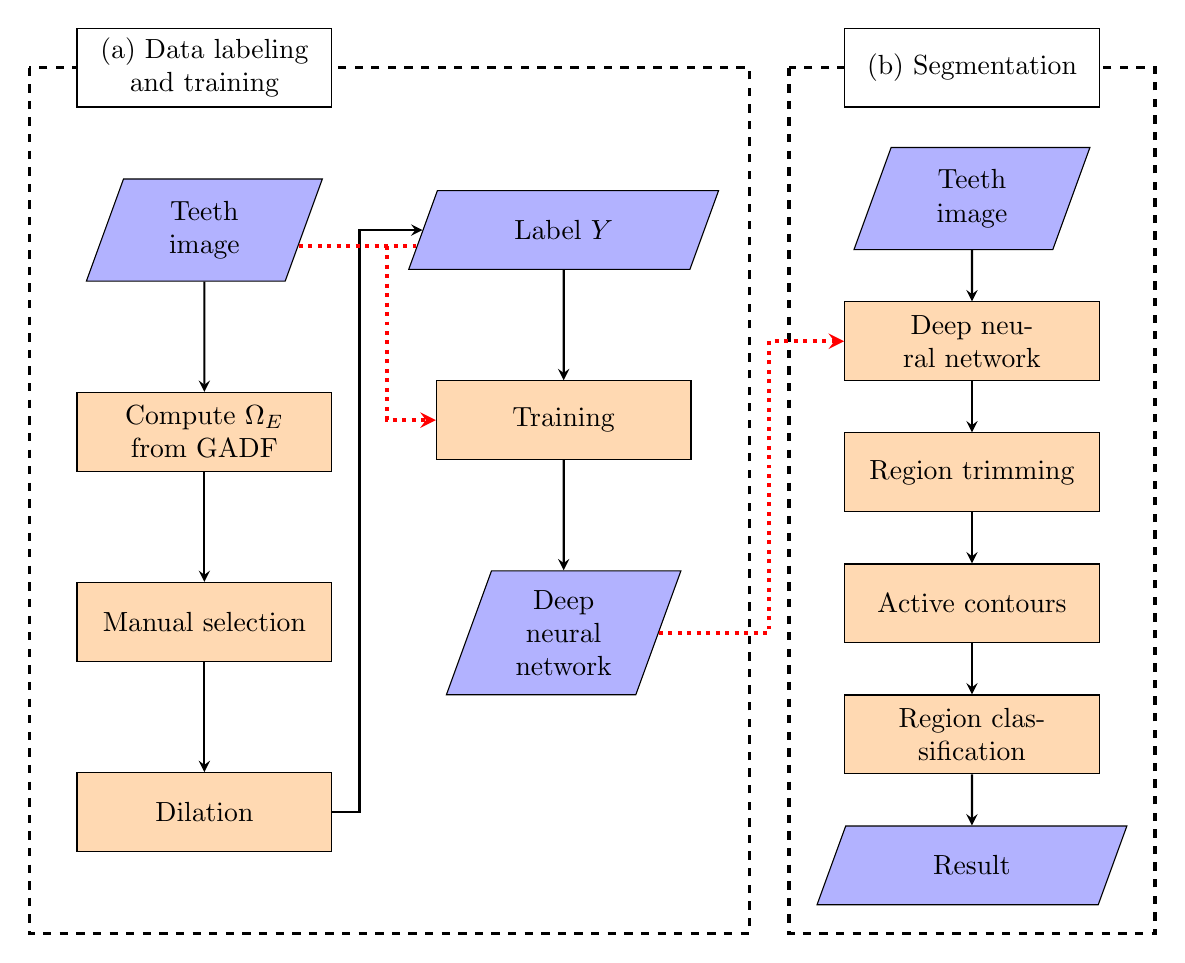
\begin{tikzpicture}[node distance=1.4cm and 1.5cm]
            \node (title1) [title] {(a) Data labeling and training};
            \node (title3) [title, right=6.5cm of title1] {(b) Segmentation};
            \node (teeth1) [io, below=.9cm of title1] {Teeth image};
            \node (pro11) [process, below=of teeth1] {Compute $\Omega_E$ from GADF};
            \node (pro12) [process, below=of pro11] {Manual selection};
            \node (pro13) [process, below=of pro12] {Dilation};
            \node (label) [io, right=of teeth1] {Label $Y$};
            \node (pro14) [process, below=of label] {Training};
            \node (dnn) [io, below=of pro14] {Deep neural network};
            
            \node (teeth3) [io, below=.5cm of title3] {Teeth image};
            \node (pro31) [process, below=.65cm of teeth3] {Deep neural network};
            \node (pro32) [process, below=.65cm of pro31] {Region trimming};
            \node (pro33) [process, below=.65cm of pro32] {Active contours};
            \node (pro34) [process, below=.65cm of pro33] {Region classification};
            \node (res) [io, below=.65cm of pro34] {Result};
            
            \draw [arrow] (teeth1) -- (pro11);
            \draw [arrow] (pro11) -- (pro12);
            \draw [arrow] (pro12) -- (pro13);
            \draw [arrow] (pro13.east) -| ($(label.west) + (-.8, 0)$) -- (label.west);
            \draw [arrow] (label) -- (pro14);
            \draw [arrow] (pro14) -- (dnn);
            \draw [arrow] (teeth3) -- (pro31);
            \draw [arrow] (pro31) -- (pro32);
            \draw [arrow] (pro32) -- (pro33);
            \draw [arrow] (pro33) -- (pro34);
            \draw [arrow] (pro34) -- (res);

            \draw [red,line width=.5mm,dotted] ($(teeth1.east) + (-.07, -.2)$) |- ($(label.west) + (-.07, -.2)$);
            \draw [arrow, red,line width=.5mm, dotted] ($(label.west) + (-.45, -.2)$) |- (pro14.west);
            \draw [arrow, red,line width=.5mm, dotted] (dnn.east) -| ($(pro31.west) + (-.95,0)$) -- (pro31.west);
            \begin{scope}[on background layer]
                \draw[black,line width=.4mm,dashed] ($(title1.west)+(-.6,0)$)  rectangle ($(title1.east)+(5.3,-11)$);
                \draw[black,line width=.4mm,dashed] ($(title3.west)+(-.7,0)$)  rectangle ($(title3.east)+(.7,-11)$);
            \end{scope}
        \end{tikzpicture}
    \end{subfigure}
    \caption{Algorithm flowchart of (a) the labeling and training and (b) segmentation process.}
    \label{Fig:flowchart}
\end{figure}
    
% Subsection: Data labeling and training strategy
\subsection{Data labeling and training by strategy}
\label{Subsec:DLT}

Labels for input data are indispensable for supervised learning. In general, labels do not accompany the data, and they should be created by human force. However, human labeling has to pay too much time and effort, and also has a big disadvantage that there is no guarantee that the label completely matches the information of the image. For example, we want to take the edge region on tooth boundary as label, and $\Omega_E$ is upon the points that exactly satisfy \eqref{Def:edge}, whereas there is no such assurance in the case of direct labeling by humans. Therefore, we devise a labeling method that reflects the information of the teeth image well while minimizing the human touch. In the left of Figure~\ref{Fig:flowchart}, algorithm flowchart of the labeling and training process are displayed. First, compute the region $\Omega_E$ where GADF faces each other and manually select connected components of $\Omega_E$ only present on the tooth boundary, let us denote the selected region $\Omega_S$. After that, the label $Y:\Omega\subset\mathbf{R}^2\rightarrow\{0,\,1\}$ is obtained as
\begin{align*}
    Y(x) = \delta_{S_\omega}(\Omega_S)\cm
\end{align*}
by the dilation $\delta_{S_\omega}$. This process can be viewed in the Figure~\ref{Fig:labeling}.

In the labeling, human did only selection process. Because of this simplicity, the label does not perfectly match the tooth boundaries. For example, the label contains unnecessary parts which are actually not related to the tooth boundary but selected because they are connected to them. And also many leakages are occurs. See Figure~\ref{Fig:4d}. 

% Figure: Experimental results
\begin{figure}[]
    \centering
    \begin{subfigure}[]{.4\textwidth}
        \centering
        \includegraphics[height=3.8cm]{./Figures/Fig4_img.pdf}
        \caption{}
        \label{Fig:4a}
    \end{subfigure}
    \begin{subfigure}[]{.4\textwidth}
        \centering
        \includegraphics[height=3.8cm]{./Figures/Fig4_er.pdf}
        \caption{$\ome$}
        \label{Fig:4b}
    \end{subfigure}\\
    \vspace{1mm}
    \begin{subfigure}[]{.4\textwidth}
        \centering
        \includegraphics[height=3.8cm]{./Figures/Fig4_seler.pdf}
        \caption{$\Omega_s$}
        \label{Fig:4c}
    \end{subfigure}
    \begin{subfigure}[]{.4\textwidth}
        \centering
        \includegraphics[height=3.8cm]{./Figures/Fig4_label.pdf}
        \caption{label $Y$}
        \label{Fig:4d}
    \end{subfigure}
    \caption{ Labeling process described in the Section~\ref{Subsec:DLT}. (a) An image in the training dataset. (b) The region $\Omega_E$. (c -- d) Manually selected region and the label obtained from dilation. }
    \label{Fig:labeling}
\end{figure}

Recent developments of deep learning approaches give us a rich intuitive to model structures how affect to its outputs. By through many researches \cite{Ronneberger:2015,Sun:2019,Wang:2019,Yuan:2020}, it is well known that the skip connections between each level of resolutions make outputs preserving small the details of labels. In general, the labels are considered fit perfectly to the data. Thus, it seems nice that the model imitates details of the label in its outputs. However, since the details in the labels are corrupted in our case, we can predict that the outputs will also have corrupted details if we train to retain all the details in the label. Therefore, to avoid not only the regions outside tooth boundary but also corrupted details in the labels, we used an encoder-decoder form of model by excluding all skip connections. On the other hand, ResNet \cite{He:2015} shows that giving identity connections to each layer plays a huge role in aspect of training process and performance. By keeping this identity connections, numerous researches provide insights by proposing models of various structures. In terms of performance, it is known that using wide or diversified layers are helpful \cite{Szegedy:2015,Szegedy:2016,Hu:2018}. In addition, by using group convolution or bottleneck structure, a lightweight model can be constructed while keeping performance \cite{Xie:2017,Li:2019}. Consequently, we uses a deep network with relatively lower latent space dimension than the input, so that the model is trained to focus more on overall aspects of labels than its details. The part of ResNeSt-50 \cite{Zhang:2020} which before the global average pooling layer is used as the encoder part, and a self-configured upscale module is used as the decoder part. The designed upscale module is shown in the Figure~\ref{Fig:network}.

% Figure: Network structure
\newcommand*{\hg}{.8}%
\newcommand*{\wid}{.4}%
\newcommand*{\hei}{2}%
\newcommand*{\init}{0}%

\begin{figure}[]
    \centering
    \begin{subfigure}[]{1\textwidth}
        \centering
        \begin{tikzpicture}
            \draw [draw=none] (\init + \hg * -1, \hei) rectangle (\init + \hg * -1 + \wid, -\hei) node (layf)[pos=.5, rotate=90, black] {\scriptsize latent variable $\ell$};
            % first
            \draw [ultra thick, gray, fill=blue!20!white] (\init + \hg * 0, \hei) rectangle (\init + \hg * 0 + \wid, -\hei) node (lay0)[pos=.5, rotate=90, black] {\scriptsize $2\times2$ trans conv, $2048$, $/2$};
            \draw [arrow] (lay0.south) -- ++(\hg - \wid, 0);
            \draw [arrow]  ($(lay0.south) + (-\hg, 0)$) -- (lay0.north);
            
            \draw [ultra thick, gray, fill=blue!20!white] (\init + \hg * 1, \hei) rectangle (\init + \hg * 1 + \wid, -\hei) node (lay1)[pos=.5, rotate=90, black] {\scriptsize $3\times3$ conv, $2048$};
            \draw [arrow] (lay1.south) -- ++(\hg - \wid, 0);
            
            \draw [ultra thick, gray, fill=blue!20!white] (\init + \hg * 2, \hei) rectangle (\init + \hg * 2 + \wid, -\hei) node (lay2)[pos=.5, rotate=90, black] {\scriptsize $3\times3$ conv, $1024$};
            \draw [arrow] (lay2.south) -- ++(\hg - \wid, 0);
            
            % second
            \draw [ultra thick, gray, fill=green!15!white] (\init + \hg * 3, \hei) rectangle (\init + \hg * 3 + \wid, -\hei) node (lay3)[pos=.5, rotate=90, black] {\scriptsize $2\times2$ trans conv, $1024$, $/2$};
            \draw [arrow] (lay3.south) -- ++(\hg - \wid, 0);
            
            \draw [ultra thick, gray, fill=green!15!white] (\init + \hg * 4, \hei) rectangle (\init + \hg * 4 + \wid, -\hei) node (lay4)[pos=.5, rotate=90, black] {\scriptsize $3\times3$ conv, $1024$};
            \draw [arrow] (lay4.south) -- ++(\hg - \wid, 0);
            
            \draw [ultra thick, gray, fill=green!15!white] (\init + \hg * 5, \hei) rectangle (\init + \hg * 5 + \wid, -\hei) node (lay5)[pos=.5, rotate=90, black] {\scriptsize $3\times3$ conv, $512$};
            \draw [arrow] (lay5.south) -- ++(\hg - \wid, 0);
            % third
            \draw [ultra thick, gray, fill=red!15!white] (\init + \hg * 6, \hei) rectangle (\init + \hg * 6 + \wid, -\hei) node (lay6)[pos=.5, rotate=90, black] {\scriptsize $2\times2$ trans conv, $512$, $/2$};
            \draw [arrow] (lay6.south) -- ++(\hg - \wid, 0);
            
            \draw [ultra thick, gray, fill=red!15!white] (\init + \hg * 7, \hei) rectangle (\init + \hg * 7 + \wid, -\hei) node (lay7)[pos=.5, rotate=90, black] {\scriptsize $3\times3$ conv, $512$};
            \draw [arrow] (lay7.south) -- ++(\hg - \wid, 0);
            
            \draw [ultra thick, gray, fill=red!15!white] (\init + \hg * 8, \hei) rectangle (\init + \hg * 8 + \wid, -\hei) node (lay8)[pos=.5, rotate=90, black] {\scriptsize $3\times3$ conv, $256$};
            \draw [arrow] (lay8.south) -- ++(\hg - \wid, 0);
            % fourth
            \draw [draw=none] (\init + \hg * 9, \hei) rectangle (\init + \hg * 9 + \wid, -\hei) node (lay9)[pos=.5, rotate=90, black] {\scriptsize bilinear, $\times2$};
            \draw [arrow] (lay9.south) -- ++(\hg - \wid, 0);
            
            \draw [ultra thick, gray, fill=orange!15!white] (\init + \hg * 10, \hei) rectangle (\init + \hg * 10 + \wid, -\hei) node (lay10)[pos=.5, rotate=90, black] {\scriptsize $3\times3$ conv, $256$};
            \draw [arrow] (lay10.south) -- ++(\hg - \wid, 0);
            
            \draw [ultra thick, gray, fill=orange!15!white] (\init + \hg * 11, \hei) rectangle (\init + \hg * 11 + \wid, -\hei) node (lay11)[pos=.5, rotate=90, black] {\scriptsize $3\times3$ conv, $128$};
            \draw [arrow] (lay11.south) -- ++(\hg - \wid, 0);
            % fifth
            \draw [draw=none] (\init + \hg * 12, \hei) rectangle (\init + \hg * 12 + \wid, -\hei) node (lay12)[pos=.5, rotate=90, black] {\scriptsize bilinear, $\times2$};
            \draw [arrow] (lay12.south) -- ++(\hg - \wid, 0);
            
            \draw [ultra thick, gray, fill=violet!15!white] (\init + \hg * 13, \hei) rectangle (\init + \hg * 13 + \wid, -\hei) node (lay13)[pos=.5, rotate=90, black] {\scriptsize $3\times3$ conv, $128$};
            \draw [arrow] (lay13.south) -- ++(\hg - \wid, 0);
            
            \draw [ultra thick, gray, fill=violet!15!white] (\init + \hg * 14, \hei) rectangle (\init + \hg * 14 + \wid, -\hei) node (lay14)[pos=.5, rotate=90, black] {\scriptsize $3\times3$ conv, $64$};
            \draw [arrow] (lay14.south) -- ++(\hg - \wid, 0);
            \draw [ultra thick, gray, fill=black!15!white] (\init + \hg * 15, \hei) rectangle (\init + \hg * 15 + \wid, -\hei) node (lay15)[pos=.5, rotate=90, black] {\scriptsize $1\times1$ conv, $1$};
            \draw [draw=none] (\init + \hg * 16, \hei) rectangle (\init + \hg * 16 + \wid, -\hei) node (layl)[pos=.5, rotate=90, black] {\scriptsize output $\hat{Y}$};
            \draw [arrow] (lay15.south) -- ++(\hg - \wid, 0);
        \end{tikzpicture}
    \end{subfigure}
    \caption{The structure of designed upscale module. Overall, each rectangle represents a trainable layer. Each layer is described by the kernel size, type, and number of channels in the output. Further descriptions like $/2$ or $\times2$ means strides or scale factor, respectively. For every trainable layers except for the last one, the outputs are produced through the batch normalization and ReLU activation function. In the last $1\times1$ convolutional layer, we uses the sigmoid activation function. }
    \label{Fig:network}
\end{figure}

% Subsection: Obtaining an edge region candidate from a neural network and region trimming
\subsection{Obtaining an edge region candidate from a neural network and region trimming}
\label{Subsec:ObtainEr}

The neural network obtained from the Section~\ref{Subsec:DLT} infers a probability map $\hat{Y}:\Omega\in\mathbf{R}^2\rightarrow\left[0,\,1\right]$ when it takes an image $I:\Omega\rightarrow\left[0,\,1\right]^3$. Here $\hat{Y}(x)$ is the probability of having an edge on tooth boundary at $x$. We call the region defined by
\begin{align*}
    \omcc = \left\{ x\in\Omega \mid \hat{Y}(x) > \alpha \right\}
\end{align*}
as an edge region candidate of $I$ and it is shown in (b) of Figure~\ref{Fig:er_cand}. One notable point is that the majority of $\omcc$ are correctly located on the tooth boundary, although the label included many unnecessary regions. 

On the other hand, $\omcc$ is not yet perfect. It contains small fragments and leakages, thus we apply a trimming process to $\omcc$ by forming closed individual tooth regions. First, small fragments and holes can be easily removed in compared to the size of $\Omega$. To deal with the leakages, it is required that figuring out where the leakages occurs. We assume that the leakages always exist with ends of $\omcc$ and thus, we can fill the leakages by finding the ends and extending them. Since $\omcc$ is a region obtained by thresholding the probability map, the thickness and shape of the region are not uniform, and so it is not easy to properly define the end. Furthermore, in order to decide which direction to extend the region at the end, the direction in which the region travels must be obtained, but it is not easy to find the direction directly from $\omcc$. By investigating to the concepts of topological skeletons \cite{Blum:1967} and 8-pixel connectivities \cite{Jonker:1992}, we were able to define ends and parametric curve which representing $\omcc$, and the problems were solved. The details are presence in Appendix~\ref{App:skeleton} and \ref{App:extend}, and in the Figure~\ref{Fig:ex_ends}, it shows the obtained ends and curves from the 8-connected skeleton. We call the resulting extended region from $\omcc$ as $\omc$.

% Figure: skeleton
\begin{figure}[]
    \centering
    \begin{subfigure}[]{.24\textwidth}
        \centering
        \includegraphics[height=3.5cm]{./Figures/Fig8_img.pdf}
        \caption{}
        \label{Fig:ex_ends_a}
    \end{subfigure}
    \begin{subfigure}[]{.24\textwidth}
        \centering
        \includegraphics[height=3.5cm]{./Figures/Fig8_curve.pdf}
        \caption{}
        \label{Fig:ex_ends_b}
    \end{subfigure}
    \vspace{1mm}
    \begin{subfigure}[]{.24\textwidth}
        \centering
        \includegraphics[height=3.5cm]{./Figures/Fig8_end.pdf}
        \caption{}
        \label{Fig:ex_ends_c}
    \end{subfigure}
    \begin{subfigure}[]{.24\textwidth}
        \centering
        \includegraphics[height=3.5cm]{./Figures/Fig8_ext.pdf}
        \caption{}
        \label{Fig:ex_ends_d}
    \end{subfigure}
    \caption{The process of finding ends and extension from the ends are appeared. (b) The parametric curves for each end (blue dots) of 8-connected skeleton are presented on $\omcc$ of the teeth image (a). (c) The ends of the region $\omcc$ are highlighted in red color and (d) extension result $\omc$.}
    \label{Fig:ex_ends}
\end{figure}

% Subsection: Segmentation using balloon shaped competing force
\subsection{Segmentation using active contours using competing ballon force}
\label{Subsec:SegLevelset}

Let $\{\Omega_i\}_{i=1}^N$ be a collection of disjoint subsets of a given domain $\Omega\subset\mathbf{R}^2$ such that
\begin{align*}
    \bigcup_{i=1}^N {\Omega_i} =\Omega\setminus\omc\pd
\end{align*}
For a purpose of finding edge, we evolves contours $C_i^{(t)}$ which is initially the boundaries of $\{\Omega_i\}_{i=1}^N$, i.e. $C_i^{(0)} = \partial\Omega_i$ for $i = 1,\,\cdots,\,N$. Suppose that we plays on a constant image which have no edge information $\Omega$. In this case, we are going to decide the edge by competing on the boundaries while protecting each other's regions. For this, we design a balloon force $fci$ competing on the interfaces using level set formulation. Let $\phi_{i,\,0}=\mbox{SDF}(\Omega_i)$, then $\fci$ is defined as:
\begin{align*}
    \fci(x,\,t) =
    \begin{cases}
        -1 & \mbox{if}\quad\phi_i(x,\,t) < 0,\\
        s\left( 1 - \sum_{j\neq i}\phi_j(x,\,t) \right) & \mbox{otherwise},
    \end{cases}
\end{align*}
where $s$ is a function which roles as the identity on positive and $0$ on negative. Observe that in the following level set formulation
\begin{align}
    \frac{\partial}{\partial{t}}\phi_i(x,\,t) &= \mu\kappa(\phi_i)\ngphii + \fci\ngphii\cm\label{Eq:compet}\\
    \phi_i(x,\,0) &= \phi_{i,\,0}\cm \nonumber
\end{align}
$\fci$ pushes $C_i^{(t)}$ outward and when it faces another contour, say $C_j^{(t)}$, both forces $\fci$ and $\fcj$ let them decide edge line without invade each other. The shape of boundary can be adjusted by the coefficient of the curvature term. Larger $\mu$ gives more forces to make the boundary flat and vice versa. In (a) and (b) of Figure~\ref{Fig:balloon_force}, the evolution processes by \eqref{Eq:compet} for several initials are shown. Furthermore, suppose that we have some barrier regions $\mathcal{B}$ defined where the contours are obstructed and cannot be crossed. Then we can consider a level set formulation:
\begin{align}
    \frac{\partial}{\partial{t}}\phi_i(x,\,t) &= \mu\kappa(\phi_i)\ngphii + \chi_{\mathcal{B}}\fci\ngphii\cm\label{Eq:compet2}\\
    \phi_i(x,\,0) &= \phi_{i,\,0}\cm \nonumber
\end{align}
which works only outside of $\mathcal{B}$. In (c) and (d) of Figure~\ref{Fig:balloon_force}, a simple example for \eqref{Eq:compet2} is in there.

For the region obtained from the Section~\ref{Subsec:ObtainEr}, we assume that there are no edge outside the region $\omc$. Following the level set evolution made from \eqref{Eq:proposed}, the each initial contour proceeds outward, and when it enters into $\omc\cap\ome$ and $\omc\setminus\ome$, then edge is determined by GADF and $F_s$, respectively. On the other hand, if neither there are no $\ome$ nor edge is not decided by $F_s$, then the inflated contours are faced each other and edge will be decided by competition between them.

% Figure: skeleton
\begin{figure}[]
    \centering
    \begin{subfigure}[]{.21\textwidth}
        \centering
        \includegraphics[height=3.1cm]{./Figures/Fig8_img1/iter0.pdf}
        \includegraphics[height=3.1cm]{./Figures/Fig8_img1/iter50.pdf}
        \includegraphics[height=3.1cm]{./Figures/Fig8_img1/iter150.pdf}
        \includegraphics[height=3.1cm]{./Figures/Fig8_img1/iter300.pdf}
        \includegraphics[height=3.1cm]{./Figures/Fig8_img1/iter800.pdf}
        \caption{}
        \label{Fig:ex_ends_a}
    \end{subfigure}
    \begin{subfigure}[]{.21\textwidth}
        \centering
        \includegraphics[height=3.1cm]{./Figures/Fig8_img2/iter0.pdf}
        \includegraphics[height=3.1cm]{./Figures/Fig8_img2/iter40.pdf}
        \includegraphics[height=3.1cm]{./Figures/Fig8_img2/iter100.pdf}
        \includegraphics[height=3.1cm]{./Figures/Fig8_img2/iter200.pdf}
        \includegraphics[height=3.1cm]{./Figures/Fig8_img2/iter300.pdf}
        \caption{}
        \label{Fig:ex_ends_b}
    \end{subfigure}
    \begin{subfigure}[]{.21\textwidth}
        \centering
        \includegraphics[height=3.1cm]{./Figures/Fig8_img3/iter0.pdf}
        \includegraphics[height=3.1cm]{./Figures/Fig8_img3/iter150.pdf}
        \includegraphics[height=3.1cm]{./Figures/Fig8_img3/iter300.pdf}
        \includegraphics[height=3.1cm]{./Figures/Fig8_img3/iter500.pdf}
        \includegraphics[height=3.1cm]{./Figures/Fig8_img3/iter1000.pdf}
        \caption{}
        \label{Fig:ex_ends_b}
    \end{subfigure}
    \begin{subfigure}[]{.27\textwidth}
        \centering
        \includegraphics[height=3.1cm]{./Figures/Fig8_img4/iter0.pdf}
        \includegraphics[height=3.1cm]{./Figures/Fig8_img4/iter250.pdf}
        \includegraphics[height=3.1cm]{./Figures/Fig8_img4/iter400.pdf}
        \includegraphics[height=3.1cm]{./Figures/Fig8_img4/iter600.pdf}
        \includegraphics[height=3.1cm]{./Figures/Fig8_img4/iter1000.pdf}
        \caption{}
        \label{Fig:ex_ends_b}
    \end{subfigure}
    \caption{From the top to the bottom, contours evolving by \eqref{Eq:compet2} are appeared with different initials and different $\mathcal{B}$. Overall contours, the different color means the different contour. (a) $\mathcal{B}=\emptyset$ and randomly located initials. (b) Circular $\mathcal{B}$ and initials inside and outside it. (c) Opened circular $\mathcal{B}$ and the same initials to (b). (d) A synthetic $\mathcal{B}$ and initials. }
    \label{Fig:balloon_force}
\end{figure}

% Subsection: Teeth and non-teeth region classification
\subsection{Teeth and non-teeth region classification}
\label{Subsec:regClass}

As a final step, classification of the segmented regions is remained. Suppose that a domain $\Omega$ of a teeth image $I$ is partitioned by the Section~\ref{Subsec:SegLevelset}. Since our goal is to segment each individual tooth, we are going to classify a teeth and a non-tooth regions and take only the tooth regions. In the human teeth image, teeth and non-tooth regions can be distinguished in terms of morphological and color information. First, while tooth have a convex-like shape, the non-tooth region has a lot of bandages on its boundary due to the shape of the roots of the teeth. Therefore, by considering the criterion $C_m < 0$ it is possible to classify regions with too many bandages on the boundary, where
\begin{align}
    C_m = \int_{\{\phi = 0\}} {\nabla\cdot\frac{\gphi}{\ngphi}}~dx\cm \label{Def:class_1}
\end{align}
and $\phi$ is a SDF of the region.

On the other hand, there is another very obvious feature of human teeth, which is that the teeth are consist of (at most) two rows, the upper and the lower jaws. Paying attention to this point, we first draw a vertical lines in each segmented region, and mark the region if there are more regions than the number of teeth row. Then, by analyzing the colors on the vertical line, the teeth and non-tooth regions can be divided. This idea is very simple but powerful. Teeth image has inhomogeneities of luminance because the human teeth are curved inward. Thus it is very hard to classify teeth and non-tooth region by directly using the global colors of image. But, under each vertical line, the points can be considered as curved inward by the same amount, and so it makes sense to analyze the colors on the vertical line and classify the regions thought the color information. In fact, classification using colors on the vertical line gives a way better result. In practice, more elaborate works are done than written here and details are provided in the Appendix~\ref{App:classVline}. 

In summary, the region classification yeld two steps: (1) The quantities in \eqref{Def:class_1} are calculated for each region, and the region with $C_m<0$ is classified as a non-tooth region. (2) The remaining region were classified using vertical lines and color information on the lines.

% Section: Experimental results
\section{Experimental results and numerical aspect}
\label{Sec:ER}

Overall experiments, parameters are fixed as $\alpha=\mu=0.5$, $\omega=\lfloor|\Omega| / 600 + 1/2\rfloor$ and $L = \lfloor\omega / 5 + 1/2\rfloor$. Basically, finite differential scheme is applied for every differentiations. For the contour evolution in \eqref{Eq:proposed}, the explicit Euler time discretization scheme is used and the computed level set function is frequently re-initialized by the scheme in \cite{SUSSMAN:1994}. In practice, the $\sko$ in the Appendix~\ref{App:skeleton} is obtained by thresholding $\ngphi < \eta$, where $\eta=\sqrt{2}/2$ rather than following the definition, and in order to reduce computing time, the skeletonization algorithm of \cite{Zhang:1984} is use before applying our algorithm to extract $\ske$ from the region $\sko$.

Training images are labeled using dedicated tool. It is designed so that a human can select a desired region simply by touching it using an input tool, such as a mouse, and this can make the actual labeling process very fast. Data augmentations in the following list are applied:
\begin{itemize}
    \item Resizing with height $\in[256,\,512]$,
    \item Patch cropping of size $256\times256$ with random location.
    \item Gaussian smoothing with $\sigma_1\in[0.25,\,0.75]$,
    \item Adding gaussian noise with $\sigma_2\in[0.005,\,0.015]$,
    \item Gamma correction with $\gamma\in[0.5,\,2]$,
    \item Horizontal flipping.
\end{itemize}
All data augmentations are randomly applied to each image with a probability of $0.5$, and each parameter was also randomly determined within the given ranges. The neural network is trained on $46$ images, by minimizing the binary cross entropy loss function using the Adam optimizer \cite{Kingma:2017}. Figure~\ref{Fig:results} shows several teeth images and its segmentation results.

% Figure: Edge region candidate and results
\begin{figure}[]
    \centering
    \begin{subfigure}[]{.3\textwidth}
        \centering
        \includegraphics[width=4.2cm]{./Figures/Fig10_img0.pdf}
        \includegraphics[width=4.2cm]{./Figures/Fig10_img1.pdf}
        \includegraphics[width=4.2cm]{./Figures/Fig10_img5.pdf}
        \includegraphics[width=4.2cm]{./Figures/Fig10_img8.pdf}
        \includegraphics[width=4.2cm]{./Figures/Fig10_img18.pdf}
        \includegraphics[width=4.2cm]{./Figures/Fig10_img17.pdf}
        \caption{Input images}
    \end{subfigure}
    \begin{subfigure}[]{.3\textwidth}
        \centering
        \includegraphics[width=4.2cm]{./Figures/Fig10_neter0.pdf}
        \includegraphics[width=4.2cm]{./Figures/Fig10_neter1.pdf}
        \includegraphics[width=4.2cm]{./Figures/Fig10_neter5.pdf}
        \includegraphics[width=4.2cm]{./Figures/Fig10_neter8.pdf}
        \includegraphics[width=4.2cm]{./Figures/Fig10_neter18.pdf}
        \includegraphics[width=4.2cm]{./Figures/Fig10_neter17.pdf}
        \caption{Edge region candidates $\omc$}
        \label{Fig:er_cand}
    \end{subfigure}
    \begin{subfigure}[]{.3\textwidth}
        \centering
        \includegraphics[width=4.2cm]{./Figures/Fig10_res0.pdf}
        \includegraphics[width=4.2cm]{./Figures/Fig10_res1.pdf}
        \includegraphics[width=4.2cm]{./Figures/Fig10_res5.pdf}
        \includegraphics[width=4.2cm]{./Figures/Fig10_res8.pdf}
        \includegraphics[width=4.2cm]{./Figures/Fig10_res18.pdf}
        \includegraphics[width=4.2cm]{./Figures/Fig10_res17.pdf}
        \caption{Segmented result}
        \label{Fig:er_cand}
    \end{subfigure}
    \caption{(a) Input images and (b) obtained edge region candidates $\omc$. The segmentation results for the images (a) are in (c).}
    \label{Fig:results}
\end{figure}

% Section: Conclusion
\section{Conclusion}
\label{Sec:Conclusion}
In this paper, we proposed a method of individual tooth segmentation in a general 2D human teeth image under the active contours framework. 
There are several obstacles interfering the segmentation process, and we have solved with appropriate image processing methods for each of them. In particular, the strong light reflections on the teeth image was a very big problem, which was solved using deep learning method. We tried to obtain candidates of edge region from the neural network, and we did this by concentrating on minimizing human touch. In addition, we proposed a force to form a balloon shaped region by competing with each other. Through this, let contours compete and decide the edge even if there is no boundary information in a local region of image.

We aimed for a collaboration between the model-based methods and the deep neural networks. In fact, it was confirmed that the two methodologies created a synergistic effect: model-based method streamline the labeling process for training neural networks using model-based methods as well as neural network simplifies the problem through inferring edge region candidate. We hope that this win-win framework will contribute to the collaborations of these two methodologies in the future.

% Section: Acknowledgement
% \section*{Acknowledgement}

%% Appendix
\appendix
% % Appendix: Prolongation from edge
% \section{Finding edges and extension from the edge}
% \label{App:prolong}

% \subsection{An 8-connected topological skelton}
% \label{Subapp:skeleton}

% The topological skeleton $\skel$ of $\omc$ can be defined in various ways that are equivalent to each other. In this paper, we use the ridge of a signed distance function:
% \begin{align*}
%     \skel = \left\{ x\in \omc \mid |\nabla\phi(x)| = 0 \right\}\cm
% \end{align*}
% where $\phi = \mbox{SDF}(\omc)$. This can be discretized in a natural way, and let $\sko$ denote it. Now consider the set of all subsets of $\sko$ whose 8-connectivities are coincide. Then we can find a maximal $\ske\subset\skel_{\omc}$ in the set such that $\forall x\in\ske$ are in only one of the two categories: (1) the connectivity of $\ske$ is changed if $x$ is removed or (2) $x$ is an end of $\ske$. Look at the Figure~\ref{Fig:ends}. Here, we define a point $x$ of a skeleton as an end if $3\times3$ window centered at $x$ is the same as one of Figure~\ref{Fig:ends}. Observe that in a $3\times3$ window of an end point of $\ske$, there are only two points end point itself and the other point. Let the end point be $x_0$ and let the other point be $x_1$. Next, in the $x_1$, there may be several points $x_0$, $x_1$ and the others. Let the set of other points be $p(x_1)$. A parametric curve $\lambda:\mathbf{Z}\cup[0,\,L]\rightarrow\Omega$ can be obtained by the Algorithm~\ref{Alg:curve}. 

% % Algorithm (Local problem for the image deblurring)
% \begin{algorithm}[]
%     \caption{Algorithm for obtaining the representative curve for $\ske$}
%     \begin{algorithmic}[]
%         \label{Alg:curve}
%         \STATE Choose $L \in\mathbf{Z}_{>0}$. Let $n=0$, $x_0\in E(\ske)$ and $x_1\in p(x_0)$.
%         \WHILE{$p_x^{(n)}==1$ or $|\lambda| < L$}
%         \STATE $\displaystyle p_x^{(n)} = p(p_x^{(n-1)}$
%         \ENDWHILE
%     \end{algorithmic}
% \end{algorithm}

% \subsection{Extension from ends}
% \label{Subapp:extend}

% Using $\gamma(t)$, we can calculate tangent and curvature at the end point and from now, we regard the ends, tangents and curvatures as of the region $\omc$. We plan to fill the leakages by trying to extend it sequentially in a more plausible direction. The basic strategy in this process is to return to the end before the extension if the leakage is not closed after a certain length of extension, and after that, start extension in the next direction. This is because we do not want to complicate the region by extensions that cannot reached, and it is assume that if the direction is appropriate, then the ends should be able to close the leakages with even a small extension. For the extension, three different cases are considered:
% \begin{itemize}
%     \item [(1)] Using $\oma$ coincident with the direction of the end.\\
%     Suppose that $\omc$ continued along an edge of an image and breaks, resulting in a leakage. If the edge is still continued even in the leakage, then $\oma$ should exist with the same direction as $\omc$. Therefore, we extend $E(\omc)$ along $\oma$ when the directions of $\oma$ and $\omc$ are similar at the $E(\omc)$, i.e.,
%     \begin{align*}
%         |T(e) \cdot F_a(e)| < \frac{1}{2},\quad e\in E(\ske).
%     \end{align*}

%     \item [(2)] Using quadratic curve.\\
%     When there are no $\oma$ with the direction at the end, then we extend the end following the quadratic curve which is the best approximation of $\gamma(t)$ in a least square sense.

%     \item [(3)] Using straight line.\\
%     Of the remaining leakages, those that can be filled with a small extension are simply extended in a straight line.
% \end{itemize}

\section{Finding edges and extension from the edge}
\label{App:skeleton}
The topological skeleton of $\omc$ can be defined in various ways that are equivalent to each other. In this paper, we use the ridge of a signed distance function:
\begin{align*}
    \skel = \left\{ x\in \omc \mid |\nabla\phi(x)| = 0 \right\}\cm
\end{align*}
where $\phi = \mbox{SDF}(\omc)$. This can be discretized in a natural way, and let the notation $\sko$ denote the discretized version. By assuming the pixel connectivities, there may exist distinct subsets of $\sko$ whose 8-connectivities are coincide. In this manner, two sets $A\subset B$ are defined to be related if
\begin{align*}
    \forall R\subset\mathcal{R}_A,\quad\exists! R'\subset\mathcal{R}_B\quad\mbox{such that}\quad C\subset D\cm
\end{align*}
and denoted as $A\sim B$. Here, $\mathcal{R}_A^8,\,\mathcal{R}_B^8$ are the set of all 8-connected components of $A$ and $B$, respectively.
Now consider a set $\calc$ defined as
\begin{align*}
    \calc = \left\{ C\sim\sko \mid \forall x\in C,\quad C\setminus\{x\} \nsim \sko \right\}\cm
\end{align*}
and let $\ske\in\calc$ be a maximal element. We call the $\ske$ as an 8-connected skelton of $\omc$. Observe that $\calc$ is a partially ordered set and so $\ske$ does not need to unique, but the existence of $\ske$ is obvious because of the trivial element of $\calc$. Look at the Figure~\ref{Fig:ends}, we define a point $x$ of a skeleton as an end if $S_3(x)$ is the same as one of the figures and let the set of all such ends be $\endske$. As seen in the figures, there are only two points, the end point itself and the other point when $x\in\endske$. Let the end point be $x_0$ and let the other point be $x_1$. If $x_1\notin\endske$, there may be several points other than $x_0$ and $x_1$ in $S_3(x_1)$. Choose $x_2\in S_3(x_1)$, the next point, to be the farthest point from $x_0$, the previous point, among the other points. By doing this repeatedly, we can obtain a parametric curve $\gamma_e:\mathbf{Z}\cap[0,\,L]\rightarrow\Omega$ given by
\begin{align*}
    \gamma_e(n) = x_n,\quad n=0,\,1,\,\cdots,\,L\cm
\end{align*}
where $e\in\endske$ and $L$ is a positive integer.

% Figure: ends of 8-conn
\newcommand*{\gsz}{.8}%
\newcommand*{\xgap}{3.2}%
\newcommand*{\ygap}{3.2}%
\begin{figure}[]
    \centering
    \begin{tikzpicture}
        \foreach \i in {0,...,3} {
            \foreach \j in {0, 1} {
                \draw [step=\gsz, black, thick, fill=black!20!white] (-\gsz * 5 + \i * \xgap, \j * \ygap) grid ($(-\gsz * 5 + \i * \xgap, \j * \ygap) + (\gsz * 3, \gsz * 3)$) rectangle (-\gsz * 5 + \i * \xgap, \j * \ygap);
                \draw [black, thick, fill=yellow!45!white] ($(-\gsz * 5 + \i * \xgap, \j * \ygap) + (\gsz, \gsz)$) rectangle ($(-\gsz * 5 + \i * \xgap, \j * \ygap) + (\gsz * 2, \gsz * 2)$);
            }
        }
        \draw [black, thick, fill=yellow!45!white] (-\gsz * 5 + 0 * \xgap, 0 * \ygap) rectangle ++(\gsz, \gsz);
        \draw [black, thick, fill=yellow!45!white] (-\gsz * 5 + 1 * \xgap + \gsz, 0 * \ygap) rectangle ++(\gsz, \gsz);
        \draw [black, thick, fill=yellow!45!white] (-\gsz * 5 + 2 * \xgap + 2 * \gsz, 0 * \ygap) rectangle ++(\gsz, \gsz);
        \draw [black, thick, fill=yellow!45!white] (-\gsz * 5 + 3 * \xgap + 2 * \gsz, 0 * \ygap + \gsz) rectangle ++(\gsz, \gsz);
        \draw [black, thick, fill=yellow!45!white] (-\gsz * 5 + 3 * \xgap + 2 * \gsz, 1 * \ygap + 2 * \gsz) rectangle ++(\gsz, \gsz);
        \draw [black, thick, fill=yellow!45!white] (-\gsz * 5 + 3 * \xgap + 2 * \gsz, 1 * \ygap + 2 * \gsz) rectangle ++(\gsz, \gsz);
        \draw [black, thick, fill=yellow!45!white] (-\gsz * 5 + 3 * \xgap + 2 * \gsz, 1 * \ygap + 2 * \gsz) rectangle ++(\gsz, \gsz);
        \draw [black, thick, fill=yellow!45!white] (-\gsz * 5 + 2 * \xgap + 1 * \gsz, 1 * \ygap + 2 * \gsz) rectangle ++(\gsz, \gsz);
        \draw [black, thick, fill=yellow!45!white] (-\gsz * 5 + 1 * \xgap + 0 * \gsz, 1 * \ygap + 2 * \gsz) rectangle ++(\gsz, \gsz);
        \draw [black, thick, fill=yellow!45!white] (-\gsz * 5 + 0 * \xgap + 0 * \gsz, 1 * \ygap + 1 * \gsz) rectangle ++(\gsz, \gsz);
    \end{tikzpicture}
    \caption{The eight candidates of the end of skeleton. The points in the skeleton are highlighted in yellow.}
    \label{Fig:ends}
\end{figure}

\section{Extension from ends}
\label{App:extend}

Now the ends and directions on the set $\omc$ are defined using the $\endske$ and $\gamma_e(t)$. The end of $\omc$ is defined by assuming that $\omc$ is cut by normal line at the $\gamma_e(L)$. The connected part of $\omc$ which contains $e$ is considered as an end of $\omc$. We can calculate tangents and curvatures of $\gamma_e$ for every $e\in\endske$ and from now, we regard the tangents and curvatures as at the end of $\ske$. We plan to fill the leakages by trying to extend it by sequentially seeking more plausible direction. The basic strategy in this process is returning to the end after a bad extension, that is, if the leakage is not closed after a certain length of extension, then return to the end and start extension in the next direction. This is because we do not want to complicate the region by extensions that cannot reached, and it is assume that if the direction is appropriate, then the ends should be able to fill the leakages with even a not very long extension. There are three different cases:
\begin{itemize}
    \item [(1)] Using $\ome$ coincident with the direction of the end.\\
    Suppose that $\omc$ continued along an edge of an image and breaks. If the edge is still continued even in the resulted leakage, then $\ome$ should exist with the same direction as $\omc$. Therefore, we extend the end along $\ome$ when the directions of $\ome$ and $\omc$ are similar at the end, i.e.,
    \begin{align*}
        |T(e) \cdot F_a(e)| < \frac{1}{2},\quad e\in E(\ske).
    \end{align*}

    \item [(2)] Using quadratic curve.\\
    When there are no $\ome$ with the same direction at the end, then we extend the end following the quadratic curve which is the best quadratic approximation of the all points of the end of $\omc$, in a least square sense.

    \item [(3)] Using straight line.\\
    The remaining leakages can be filled with an extension along the best linear approximation in a least square sense.
\end{itemize}

% Appendix: Region classification
\section{Region classification using vertical lines}
\label{App:classVline}
Suppose that a domain $\Omega$ of a teeth image $I$ is partitioned by the \ref{Subsec:SegLevelset}. Let $x$ is a point in a member of partition of $\Omega$ and let $V(x)$ be a vertical line through the point $x$. Since human teeth have only two teeth, upper and lower, it can be assumed that non-tooth regions exist only when there are three or more regions through which $V(x)$ passes, and let those regions be $\{\omi\}_{i=1}^N$. We try to classify these regions as whether they are teeth or not using color information. However, since human teeth are curved, the distance between the camera and each tooth is not constant even in one image. Since the brightness and color of the image vary according to the degree of curved from the front, classification through color information for the entire region cannot be easily achieved. In this circumstance, we can assume that the teeth below the line curve to a similar degree from the front, so it makes sense to analyze the colors at $V(x)$ and classify the regions thought $V(x)$. In general, human teeth and neighbor parts are usually considered as white and red, respectively but teeth contain a lot more yellow than expected, which is due to contaminants on the tooth surface. Thus we moved from RGB space to CIELAB \cite{Zeileis:2009} color space to effectively separate the three colors, white, red and yellow. Let us denote the image represented to CIELAB as $I_{LAB}=(I_L,\,I_a,\,I_b)$. Here the $k$-means clustering algorithm is used. The important parameter for the $k$-means algorithm is setting initial seeds on which the algorithm start clustering. We set a total of three initial points, each to start close to white teeth, yellow teeth, and the other relatively red parts. The detailed initial points $p_1,\,p_2,\,p_3$ are as follows:
\begin{align*}
    p_1 = (100, 0, 0)\cm\quad p_2 = I_{LAB}(a^*)\cm \quad  p_3 = (50,\,0,\,\max(I_b))\cm
\end{align*}
where $a^* = \mbox{argmax} I_a$. In practice, there are $50\%$ of points are used for each member of partition of $\Omega$ and class of the member is determined by the votes of each point.

%% References
\bibliographystyle{siam}
\bibliography{bibliography}

\end{document}
